\chapter{Machine learning}
\label{chap:backml}

\begin{overview}{Overview}
The goal of this chapter is mainly to give some keys to understand our contributions to a reader with basic knowledge of \acrlong{ml}. It is not aimed at being a thorough presentation of the field or of the different methods but rather an overview. For the readers who would still like to deepen their knowledge about these methods, we provide pointers to relevant litterature. In this chapter, we also introduce the notations that we use throughout this thesis. 

Section \ref{sec:backml:whatisml} provides a short definition of \acrlong{ml} and a first example of an \acrshort{ml} problem. Section \ref{sec:backml:families} explores the different ways the field of \acrlong{ml} can be structured (\eg supervised vs. unsupervised learning, classification vs. regression, classical machine vs. deep learning...) in order to position our work in its context.   
\end{overview}

\section{What is machine learning ?} 
\label{sec:backml:whatisml}

A computer program is said to learn from experience $E$ with respect to some class of tasks $T$ and performance measure $P$, if its performance at tasks in $T$, as measured by $P$, improves with experience $E$ \parencite{mitchell1997machine}. Machine learning concerns the study of such programs, commonly referred to as \textit{models}, and how to build them by learning. A \textit{model} $h$ can be seen a function taking an input $\vect{x} \in \mathcal{X}$ (\aka observation, example, instance) and producing an ouput $h(\vect{x})$ or $\hat{y} \in \mathcal{Y}$. Entities $\vect{x}$ and $h(\vect{x})$ can be  n-dimensional tensors and encode many kind of data types: data record, image, graph, time series, text... When $\vect{x}$ is a vector, its components are commonly called \textit{features} or \textit{variables}. A model can have several inputs (\resp outputs) in which case $\vect{x}$ (\resp $y$) is a $n$-tuple.

In \acrlong{ml}, a model is built by a \textit{learning algorithm}. Formally, a learning algorithm is defined by a set $\mathcal{H}$ of candidate models called the \textit{hypothesis space}, a performance measure $P$ for a model and an optimization strategy. As input, the algorithm is provided with \textit{training data} (the experience $E$, \aka learning or training set) that it uses to build, optimize and evaluate the model. The algorithm output is a model $h \in \mathcal{H}$ that maximises the performance criterion. 

As an example, a common task is \textit{natural image classification} where the model must assign a label to a picture. For instance, one would want to detect whether a picture contains a human, an animal or an inanimate object. In this case, considering that the images are encoded with integers, the input space is the set of all possible color images: $\mathcal{X} \subset \mathbb{N}^{h\times w\times c}$ where $w$, $h$ and $c$ are respectively the image width, height and number of channels (which equals to 3 in RGB color images). The output space contains the 3 labels of interest: $\mathcal{Y} = \left\{\textit{human}, \textit{animal}, \textit{object}\right\}$. The model would take an image $\vect{x} \in \mathcal{X}$ as input and, based on its content, output $\hat{y}$, one of the predefined labels. This label $\hat{y}$ might be false if the model makes a mistake. Therefore, for the sake of distinction, the correct label is denoted $y$ (\aka ground truth). As a performance measure $P$, one could assess the correctness of the ouput label by assigning 0 to correct predictions and 1 to errors. This performance measure is called the \textit{zero-one loss} and is written as:

\begin{equation}
\ell_{0-1}(y, \hat{y}) = \mathbb{1}_{y\neq\hat{y}}
\end{equation}

There are numerous tasks beyond natural image classification to which \acrlong{ml} can be applied nowadays. In the next sections, we will discuss some of them and dive a little deeper into algorithms and topics related to learning which are relevant to this thesis.


\section{Families of learning methods}
\label{sec:backml:families}

There are many ways to structure the ecosystem of \acrlong{ml} methods. This section explores some of them.

\subsection{Supervised learning}
\label{ssec:backml:sl}

\textit{Supervised learning} (\acrshort{sl}) regroups methods where the learning process is guided by an output signal. We formalize a supervised task as the tuple $\left(\mathcal{X}; \mathcal{Y}; p(\vect{x}, y)\right)$ where $\mathcal{X}$ and $\mathcal{Y}$ are respectively the input and output spaces and $p(\vect{x}, y)$ is a probability distribution over those joint spaces. The learning algorithm is provided with a training set 
\begin{equation}
\label{eqn:backml:supervised}
\left\{(\vect{x}_i, y_i) \mid i = 1,...,n ; (\vect{x}_i, y_i) \sim p(\vect{x}, y) \right\}
\end{equation}
where $y_i \in \mathcal{Y}$ is the output signal for the observation $\vect{x}_i \in \mathcal{X}$. The learning algorithm objective is to find a model $h \in \mathcal{H}$ that approximates at best the output. 

When the output space is a finite set of discrete scalar values $\mathcal{Y} = \left\{1, 2, ..., C\right\}$, the problem is called \textit{classification}. $C$ denotes the cardinality of the set $\mathcal{Y}$ or the number of classes. When $C = 2$, the problem is said to be \textit{binary}. In classification, the model should predict the most probable output class given an example:
\begin{equation}
\hat{y}_i = \argmax{y_k \in \mathcal{Y}} p(y=y_k|\vect{x}=\vect{x}_i)
\end{equation}
Examples of classification tasks are for instance assigning a label to an image or detecting whether an email is a spam or not. 

When the output space is continuous and the output is a real scalar value, the problem is called \textit{regression}. In this case, the model should predict the expected value $y$ given any input $\vect{x}_i$:
\begin{equation}
h(\vect{x}_i) = \mathbb{E}\left[y|\vect{x}=\vect{x}_i\right]
\end{equation}
Examples of regression problems are trying to predict the price of a house given its area, the amount of product generated by a factory in a given time period or the review score of a product on an e-commerce platform. 

Beyond scalar outputs, some models sometimes predict structured outputs. This is the case for \textit{image segmentation} which focuses on classifying each pixel of an image (\ie what kind of object does this pixel belong to in the image?). The output of the model is a segmentation mask where pixel at row $i$ and column $j$ is classified as $\hat{y}_{ij} \in \mathcal{Y}$. For some tasks, a mask is not always necessary, one is rather interested in the coarse location of the objects. This kind of task is called \textit{detection} where the output of the model, the location, can be encoded as image coordinates $(i, j)$ representing the object's center of gravity or any of its point. Another common representation is the bounding box, a box containing exactly the object of interest, encoded by the position of a corner of the box in the image and its height and width.

In \acrlong{sl}, the training signal is often created by humans by manually annotating examples. Such guidance allows to use well-studied methods and usually helps learning strong models but also comes at a cost because of the human intervention. This is especially aggravated when the target task is difficult as, the more complex, the more data is required to sample sufficiently the input space. In some domains, annotations are particularily cumbersome to obtain because one lacks raw data, or because the annotation process requires the intevention of experts (\eg medical data). In this case, this issue is referred to as \textit{data scarcity}. In general, the lack of data hampers the successful application of \acrlong{sl} but several approaches exist to work it around which are presented briefly in the following sections. 

\subsection{Unsupervised learning}
\label{ssec:backml:usl}

In opposition to \acrlong{sl}, \acrfirstit{usl} regroups methods where no output signal is provided to guide the learning process. The learning algorithm is provided with 
\begin{equation}
\left\{\vect{x}_i \mid i = 1,..., n ; \vect{x}_i \sim p(\vect{x})\right\}
\end{equation} 
and attempts to extract information from this dataset. A common unsupervised task is \textit{density estimation} where the goal is to model the generating distribution $p(\vect{x})$ but there also exists other types of methods. For instance, \textit{clustering} where the algorithm searches for natural groups of observations or features. Another example is \textit{dimensionality reduction} where the algorithm projects high-dimensional data into a lower-dimensional space while attempting to preserve as much information as possible. An interested reader will find more information about these methods in \parencite{friedman2017elements}. There exists another family of \acrlong{usl} methods that was first explored in the 1980s with autoencoders but has gained much traction recently. It is called \textit{self-supervised learning} \parencite{lecun2021self}. The idea behind this family of methods is to exploit supervised learning algorithms but rather than guiding the learning process with human annotations, the training signal is found in the data itself. An example of such methods is \textit{image reconstruction}. Random parts of the input images are truncated (\eg replaced by black squares) and the model must be able to re-generate the truncated parts. In this case, input and output signal are respectively the original and the truncated image. The model input can be generated from the original data without human intervention. 

\subsection{Between supervised and unsupervised learning}
\label{ssec:backml:inbetween}

The families discussed in Sections \ref{ssec:backml:sl} and \ref{ssec:backml:usl} do not cover all the existing \acrlong{ml} methods but are rather at the ends of a spectrum. There also exists intermediate families of methods. Halfway between supervised and \acrlong{usl} is \acrfirstit{ssl} which focuses on methods that use a dataset where only a part of the observations have an associated output signal. The dataset is composed of two subsets:
\begin{eqnarray}
S_a = \left\{(\vect{x}_i, y_i) \mid i = 1,...,n_a; (\vect{x}_i, y_i) \sim p_{\mathcal{X},\mathcal{Y}}; \vect{x}_i \sim p_a(\vect{x})\right\} \\
S_u = \left\{\vect{x}_i \mid i = 1,...,n_u; \vect{x}_i \sim p_u(\vect{x})\right\}
\end{eqnarray}
These  methods make some assumptions about the ``closeness'' of the input distributions $p_a(\vect{x})$ and $p_u(\vect{x})$ \parencite{chapelle2006semi} which allow to exploit both sets to solve some particular tasks. One of the earliest forms of \acrlong{ssl} is \textit{self-training} where the model is initially trained in a supervised manner on the set $S_a$, then iteratively refined by using both $S_a$ and $S_u$ as training data until a certain quality criterion is met. In order to use the second set, an output signal is predicted for all samples of $S_i$ with the model being trained. 

Closer to \acrlong{sl} is \acrfirstit{wsl} which focuses on methods where the annotations are noisy (\eg $y$ can be incorrect or imprecise), coarse or incomplete (similar to \acrlong{usl}\TODO{check any diff with usl}). The challenge of working with coarse annotations consists in having a model output $h(\vect{x})$ that contains more information than the training signal $y$. Coming back to our example of Section \ref{sec:backml:whatisml}, a weakly-supervised problem would consist in locating the human, animal or object in the image using only the label as training signal.


\subsection{Shallow versus deep learning}

Many things in our world can be viewed as hierarchies of concepts. For instance, a human body is composed of body parts like a head. The head includes the face which is itself composed of several elements: cheeks, eyes, nose, \etc. This decomposition could be refined even more and could also be applied to other concepts. Understanding hierarchies is sometimes key to learn some concepts efficiently. In computer vision, for example, an image can be seen as a hierarchy going from the actual objects it contains down to the pixels. Direct interpretation of individual pixels is rarely enough for learning anything meaningful. However, pixels combined together make edges, which themselves make textures, which are eventually combined in several rounds to reach meaningful semantic elements (see Figure \TODO{add figure to illustrate hierarchy of concept}). Therefore, being able to understand this hierarchy is a first step towards image understanding.   

Most of the \acrlong{ml} methods developed until recently can arguably be considered ``\textit{shallow}'' which means that they are not complex enough (\eg a linear model) or their learning process is not adapted (\eg a decision tree) to learn or exploit such hierarchies. In order to successfully apply these methods to complex data with hierarchical structure, one usually needs to help the learning algorithm by pre-processing the data and extract meaningful information using field knowledge. This process is called \textit{manual feature extraction} or \textit{engineering} and has been an important part of the application of machine learning algorithms. In computer vision, a great body of work is focused on creating complicated pipelines of feature extraction that produce hundreds of different features that can be used to understand images and alleviate the problem (\eg SURF \parencite{bay2006surf}, ORB \parencite{rublee2011orb}). However, more recently methods based on neural networks have shown that manual feature extraction was usually not the best performing approach for a wide variety of tasks.

In 2012, the third iteration of a \acrlong{ml} challenge called ImageNet \parencite{russakovsky2015imagenet} was organized. One of the tasks was image classification and all but the best methods used combinations of shallow learning algorithms and features extraction. The winning method \parencite{krizhevsky2012imagenet} however did not and instead used a deep convolutional neural network trained on the raw images. They beat the second best method by a margin of 11\% error rate. This extraordinary improvement revived the interest of the \acrlong{ml} community to neural networks and launched ``\acrlong{dl}''. Nowadays, it is a bit clearer why the winning method (\ie the AlexNet architecture) worked so well. Indeed, in its design, the deep neural network incorporates some particularily beneficial \textit{inductive bias}, a set of assumptions that narrow the search of a good model in the hypothesis space. This inductive bias includes a trainable multi-layered structure that can automatically learn hierarchical concepts from the data directly. In other words, instead of manual feature engineering, features are learned automatically. Section \ref{sec:backml:deeplearning} dives a little further into deep learning concepts relevant to this thesis.

\subsection{Transfer learning}
\label{ssec:backml:transfer}

As humans, we have extraordinary learning capabilites. Throughout our lives, we learn to move, communicate, interact with our environments and more. One specific learning ability that we possess is to use knowledge we have acquired in a given context to learn faster in a different context. For example, someone who already plays the violin will probably feel it easier to learn to play the piano than someone who has no music education at all. In a way, we ``transfer'' knowledge and skills from a task to another. 

This idea has been applied in \acrlong{ml} and from this application emerged \acrfirstit{tl} \parencite{yang2020transfer}. This field studies the ways knowledge learned from one or more tasks, called the \textit{source tasks}, can be exploited to learn more effectively on another task, the \textit{target task}. This subject has been researched for few decades now, as the first contributions about \acrlong{tl} date back to the end of the 1970s \parencite{bozinovski2020reminder}. A surge of interest happened in the 1990s notably with a NIPS-95 workshop called ``\textit{Learning to Learn: Knowledge Consolidation and Transfer in Inductive Systems}'' which discussed the importance of retaining previously-learned information for efficient learning. Since then, the interest has only been growing and the emergence of \acrlong{dl} has created new possibilities for \acrlong{tl}. 

Transfer learning methods are organized based on the properties of the source and target tasks. The different types of supervision (or lack thereof) discussed in Sections \ref{ssec:backml:sl} and \ref{ssec:backml:usl} also apply for \acrlong{tl} in which case the supervision qualifier relates to the target task only. For instance, in supervised \acrlong{tl}, the target task is a supervised dataset as described in Equation \ref{eqn:backml:supervised}. For the remainder of the section, we will assume that the source tasks are also supervised. 

Transfer learning can be \textit{homogeneous} (see Definition \ref{def:backml:homotransfer}) when the source and target tasks only differ by the distributions of their data. As an example, let us suppose we would want classify pictures taken with a camera equipped with a certain sensor (dataset $B$) and that we also have at hands another dataset of pictures taken with a camera equipped with another type of sensor (dataset $A$). Each captor has a certain noise pattern which results in dataset $A$ and $B$ to have a slighlty different distributions in the pixel intensities (\ie $p_A(x) \neq p_B(x)$). This specific setup where only the inputs distributions differ is also called \textit{domain adaptation}.  

\begin{definition}
\label{def:backml:homotransfer}
Transfer learning between a source task $\left(\mathcal{X}_{s}, \mathcal{Y}_{s}, p_{s}(\vect{x}, y)\right)$ and a target task $\left(\mathcal{X}_t, \mathcal{Y}_t, p_t(\vect{x}, y)\right)$ is said to be \textbf{homogeneous} when $\mathcal{X}_s \cap \mathcal{X}_t \neq \emptyset$ and $\mathcal{Y}_s = \mathcal{Y}_t$ but $p_s(\vect{x}) \neq p_t(\vect{x})$ or $p_s(y|\vect{x}) \neq p_t(y|\vect{x})$. 
\end{definition}

Transfer learning can be \textit{heterogeneous} (see Definition \ref{def:backml:heterotransfer}). An example that will be addressed later in this thesis is the transfer of a model trained for natural image classification to medical image classification. In this case, the tasks are different as the first consists in identifying the presence of a type of object in the image whereas the other consists in assessing the malignancy of a tumor from an image of a tissue. The input distributions also differ as medical images have completely different content and appearance.  

\begin{definition}
\label{def:backml:heterotransfer}
Transfer learning between a source task $\left(\mathcal{X}_{s}, \mathcal{Y}_{s}, p_{s}(\vect{x}, y)\right)$ and a target task $\left(\mathcal{X}_t, \mathcal{Y}_t, p_t(\vect{x}, y)\right)$ is said to be \textbf{heterogeneous} when $\mathcal{X}_s \cap \mathcal{X}_t = \emptyset$ and/or $\mathcal{Y}_s \neq \mathcal{Y}_t$.
\end{definition}

When the decision to apply \acrlong{tl} has been taken, remains the choice of the transfer approach. Based on how they operate, \parencite{yang2020transfer} have identifed four different categories of \acrlong{tl} algorithms: 

\begin{enumerate}
  \item \textit{instance-based}: knowledge transferred corresponds to the weights attached to the source examples,
  \item \textit{feature-based}: knowledge transferred corresponds to the subspace spanned by the features in the source and target domains,
  \item \textit{model-based}: knowledge to be transferred is embedded as a part of the source domain models,
  \item \textit{relation-based}: knowledge to be transferred corresponds to rules specifying the relations between the examples in the source domain. 
\end{enumerate}

Transfer learning performance is influenced by serveral factors including how well the method is able to capture and use transferrable knowledge. The task-relatedness is also an important factor: usually the more similar the tasks, the better the performance. Sometimes, performance are worsen by the use of transfer learning. This happens for instance when the source and target tasks are not related enough. Moreover, the training process on the target task can cause some of the previously-learned knowledge to be lost as most \acrlong{ml} methods do not have a memory mechanism to retain such information. These two phenomena are respectively called \textit{negative transfer} \parencite{zhang2020overcoming} and \textit{catastrophic interference} \parencite{french1999catastrophic}. Although some methods have been proposed to tackle these challenges, how to anticipate and correct them are still open research questions.

\subsection{Multi-task learning}
\label{ssec:backml:mtl}

In \acrlong{tl}, the transfer process happens in two steps. First, knowledge is extracted from the source tasks one way or another, then later used for learning the target task. A similar approach is \acrfirstit{mtl} where, rather than performing the transfer in two steps, everything happens at once: a model is trained on all tasks simultaneously. Compared to learning each task individually, this approach has several advantages: it increases the total amount of data available for training a model, a more robust and universal representations can be learned by sharing knowledge between tasks and, to a certain extent, it prevents the model to overfit a specific task\footnote{See more on overfitting in Section \ref{ssec:backml:bvtradeoff}.}. In the best scenarii, the use of \acrlong{mtl} improves the performance of each individual task compared to a setup where the tasks are treated independently. In opposition, it happens that antagonistic tasks cause the resulting individual task performance to be worse. This issue is related to negative transfer and catastrophic interference introduced in Section \ref{ssec:backml:transfer}. 

Similarily to \acrlong{tl}, \acrlong{mtl} methods can be either \textit{heterogeneous} when the tasks are of different types (\eg supervised, unsupervised, classification, regression), or \textit{homogeneous} when tasks have only one type. In supervised \acrlong{mtl}, \parencite{zhang2017survey} have identified three families of methods:

\begin{enumerate}
  \item \textit{feature-based}: share knowledge through learning features common among the tasks
  \item \textit{instance-based}: identify useful data instances and share knowledge through these intances
  \item \textit{model} or \textit{parameters-based}: use learned models as proxies to extract information about tasks relatedness
\end{enumerate}


% ===================
% Eval and selection
% ===================
\section{Model evaluation and selection}

As stated in Section \ref{sec:backml:whatisml}, evaluation is a core principle of \acrlong{ml} as a learning algorithms should select a model that maximizes a performance criterion. In this section, we introduce different concepts related to the evaluation and selection of machine learning models. In Sections \ref{ssec:backml:bvtradeoff} and \ref{ssec:backml:bvtradeoff}, we discuss the importance of generalization for \acrlong{ml} models and the related topics of bias-variance trade-off and overfitting. In Section \ref{ssec:backml:modelselection}, we discuss further practical consideration related to model selection. In Section \ref{ssec:backml:metrics}, we finally introduce different metrics used in this thesis. 


\subsection{Empirical risk minimization}
\label{ssec:backml:modelselection}
As stated in the introduction, the objective of a learning algorithm is to find a model $h \in \mathcal{H}$ that maximizes a performance measure or, alternatively, minimize a risk which can be formalized as the expected risk (for a supervised problem) \parencite{vapnik1992principles}:

\begin{equation}
\label{eqn:backml:expriskmin}
R(h) = \mathbb{E}_{\mathcal{X},\mathcal{Y}}\left\{\ell\left(h(\vect{x}), y\right)\right\}
\end{equation}

where $\ell: \mathcal{Y}\times\mathcal{Y} \rightarrow \mathbb{R}$ is a loss function which measures the closeness between $h(\vect{x})$ and $y$. The expected risk is also called the \textit{generalization error}. The model that minimizes $R(h)$ is therefore the best possible model for the task and is called the Bayes model $h_B$. In practice, it is rarely possible to directly minimize the expected risk as one does not have access to the true distributions. It is therefore more convenient to work with an unbiased estimator of the estimated risk, the empirical risk, which is evaluated using the available supervised training set $\mathcal{S}$:

\begin{equation}
\label{eqn:backml:empiricalrisk}
R_e(h) = \frac{1}{n} \sum_{i=1}^{|S|} \ell(h_\mathcal{S}(\vect{x}_i), y_i), (\vect{x}_i, y_i) \in \mathcal{S}
\end{equation}

The \acrfirstit{erm} principle suggests that a learning algorithm should pick a model that minimizes the emprical risk in order to approximate $h_B$ as well as possible. Most machine learning algorithms apply this principle.

\subsection{Bias-variance trade-off and overfitting}
\label{ssec:backml:bvtradeoff}

Whereas it can be shown that the empirical risk, under some assumptions, converges to the expected risk when the training set grows ($n \rightarrow \infty$), in practice, one does not have access to an infinitely-large dataset. Therefore, the learned model will often differ from $h_B$ and its expected risk will often be larger. The effect of the ``\textit{choice}'' of a finite training set on the error can be studied using the \textit{bias-variance decomposition} of the error \parencite{geman1992neural, geurts2009bias, friedman2017elements}:

\begin{equation}
\label{eqn:backml:biasvariancedec}
\mathbb{E}_{LS}\left\{\mathbb{E}_{\mathcal{X},\mathcal{Y}}\left\{ \ell(h_{LS}(\vect{x}), y)\right\}\right\} = \text{noise}(\vect{x}) + \text{bias}^2(\vect{x}) + \text{variance}(\vect{x})
\end{equation}

where $\mathbb{E}_{LS}$ is the expectation over all training sets of size $n$ that can be extracted from $p(\vect{x},y)$ and $h_{\mathcal{S}} \in \mathcal{H}$ is the model learned from learning set $\mathcal{S} \in LS$. The \textit{noise} term is the error of $h_B$ and is therefore irreductible. The \text{bias} is the difference between $h_B$ and the average model (over models generated from $LS$). The \textit{variance} measures the variability of the predictions around the average model caused by the training set randomness. Several elements have a direct impact on these error terms such as: model capacity, training set size, noise in the data, \etc. 

The \textit{capacity} or \textit{complexity} of a model is related to its ability to capture complex relationships in the data. Linear models are examples of low-capacity models as they are only able to capture linear relationships. Non-linear models such as random forests (see Section \ref{sec:backml:treebased}) or deep neural networks have a higher complexity or capacity compared to linear models. 

Low-capacity models usually have low variance as their limited expressiveness does not allow them to change much based on the training data but they also have high bias as failing to capture complex relationships prevents the model from approximating $h_B$ correctly, this is \textit{underfitting}. In opposition, high-capacity models have low bias as their expressiveness allow them to approximate $h_B$ more accurately but this expressiveness also leads to high-variance as the model can learn a function which is too expressive compared to $h_B$ and, even worse, can fit the noise in the training data. This phenomenon is called \textit{overfitting} and hampers the models ability to generalize. The \textit{bias-variance trade-off} results from these observations and states that finding a good model (or minimizing the expected risk) consists in finding the trade-off between low- and high-capacity or underfitting and overfitting. In Figure \ref{fig:backml:biasvariancetradeoff} is plotted the classical representation of this trade-off.\TODO{what about the empirical risk in this setting ? in plot ?}

\begin{figure}
  \centering
  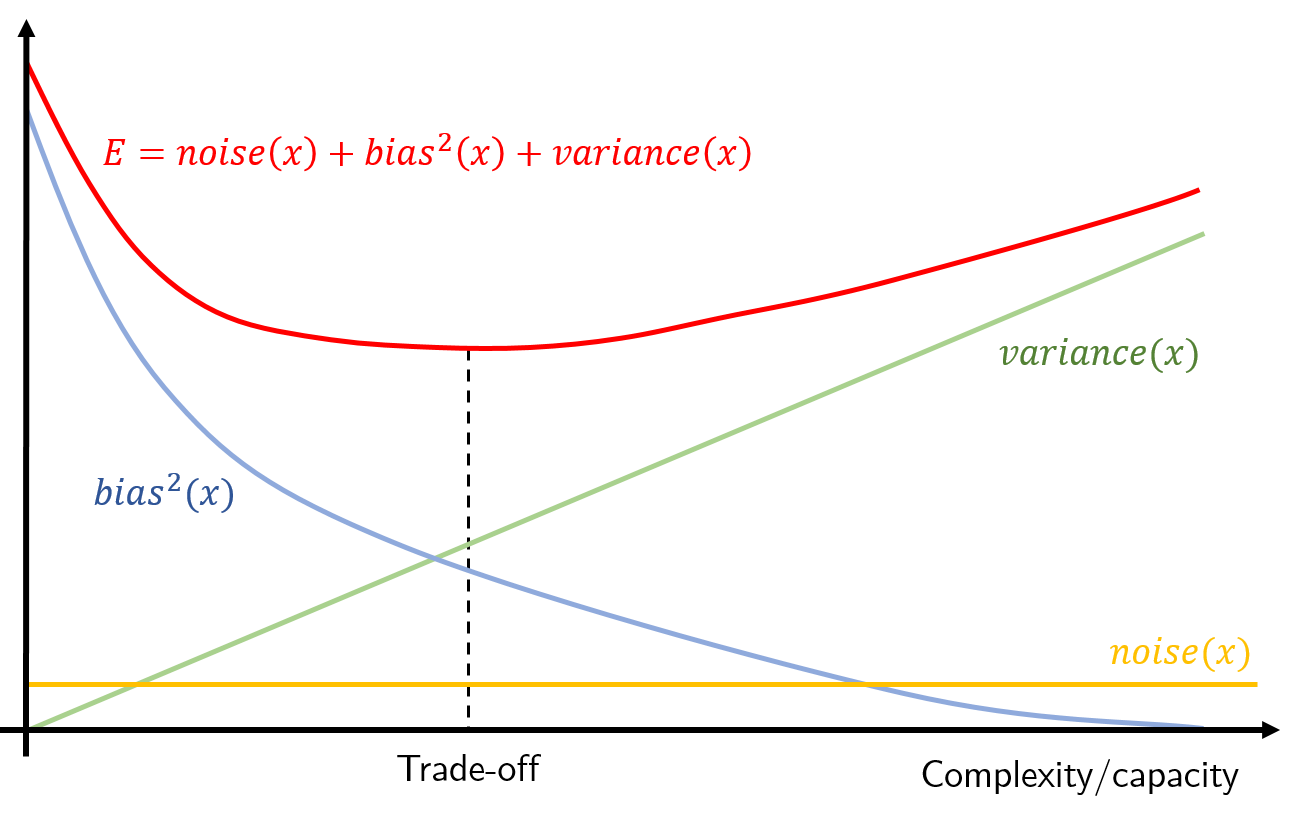
\includegraphics[scale=0.5]{backml/biasvariancetradeoff.png}
  \caption{The bias-variance trade-off illustrated.}
  \label{fig:backml:biasvariancetradeoff}
\end{figure}

\subsubsection{Over-parametrized models}

With the advent of \acrlong{dl}, model complexity has exploded as typical \acrlong{dl} models have millions or even billons of parameters (see Section \ref{ssec:backml:dlarchi}). The bias-variance trade-off tells us that these models should be extremely prone to overfitting but the reality is different. Typically, it is not uncommon to find tasks for which deep learning models reach an empirical risk close to zero but actually generalize well to unseen data \parencite{zhang2021understanding}. Although the models are able to basically memorize the training data, the learned function is actually very robust. This phenomenon is currently being investigated and several explanations have been proposed such as the deep double-descent \parencite{belkin2019reconciling}. \TODO{check if more to say + add plot}

\subsection{Model selection and evaluation in practice}

These considerations have direct consequences on practical applications of machine learning. In particular, the presence of overfitting causes the empirical risk to reflect poorly the generalization error of a model. There are two common tasks where using the empirical risk only is not reliable which are \textit{model selection} and \textit{model evaluation}. The former consists in finding the model that would generalize best among a set of candidates and the latter consists in evaluating the expected performance of a model when it will be used on new data. Both tasks involve evaluating the generalization of a model. There exists several approaches to solve these tasks. 

The simplest one is the use of an independant test set: the source dataset is split into two subsets, the train and test sets, which are used to respectively train and evaluate the model. The size of the subsets should be made such that the train set is large enough for the model to be able to learn but the test set should be large enough for the estimate of the error to be reliable. Those two objectives are obviously antagonistic. Moreover, this approach is not viable if the source dataset is too small as reducing even more the size of the sets will make both the training and evaluation unreliable. The test-set approach actually evaluates the generalization error of the model for the given dataset but not the expected generalization error used in Section \ref{ssec:backml:bvtradeoff}.

Another approach that actually estimates the expected generalization error is \acrfirstit{cv} which simply repeats the train-test approach with different splits of the source dataset. For each train-test split, a model is trained on the train set and evaluated on the test set. The \acrlong{cv} score is computed by averaging the test scores of all splits. There exists several approaches for \acrlong{cv} whhich differ by how they generate their splits. A common approach is \textit{$k$-fold \acrlong{cv}} where the data is randomly split into $k$ subsets and each subset is selected in turn to be the test set (and the remaining folds make the train set). 

An important consideration is to never use a model selection score as the evaluation score of a model. Indeed, optimizing the choice of a model usually results in the selection score to be an overly optimistic estimator of the generalization performance of the model. In practice, this results in a three-way split of the training dataset: one extracts some train, validation and test sets. The models are trained on the first, selected on the second and the final model is evaluated on last. When the dataset is too small for such a three-way split, a common approach consists in extracting a test set from the initial dataset and then performing \acrlong{cv} on the train set. As a general rule, every decision influenced one way or another by the output $y$ should be done within a validation loop to avoid overfitting (using either \acrlong{cv} or an independant test-set).

These two approaches are based on a strong assumption that the extracted sets are independant. If they are not, this would most probably lead to overfitting and the resulting selection or evaluation scores being overly optimistic. Therefore, it is sometimes not enough to split the sets randomly and domain knowledge must be used during the splitting procedure to enforce sets independance. This issue is sometimes called \textit{data leakage} \parencite{kaufman2012leakage} as information ``leaks'' between the sets. This topic will be discussed in Section \ref{sec:backdp:dataset} as \acrlong{dp} datasets must treated carefully to avoid this issue. 

\subsection{Metrics}
\label{ssec:backml:metrics}

% F1 ?
The metrics presented in this section are mostly supervised classification performance measures. Given a supervised dataset as described in Equation \ref{eqn:backml:supervised}, the metrics evaluate how the predicted class $\hat{y}_i$ compares to the ground truth class $y_i$. In the remainder of the thesis, when the higher the better for a metric, we will call it a \textit{score}. In opposition, when the lower the better, we will call it a \textit{loss}. In terms of notations, a loss and a score computed over a set of data will respectively be noted $\mathcal{L}$ and $\mathcal{M}$.

\subsubsection{Accuracy}
\label{sssec:backml:metric:acc}
The accuracy was introduced in our first example of a machine learning problem in Section \ref{sec:backml:whatisml} with its dual, the zero-one loss. The accuracy assigns 1 to correct predictions and 0 to misclassified samples. The accuracy score can be computed over a dataset:

\begin{equation}
\label{eqn:backml:accuracy}
\mathcal{M}_{\text{acc}} = \dfrac{1}{n} \sum\limits_{i = 1}^n (1 - \ell_{\text{0-1}}(y_i, \hat{y}_i))
\end{equation} 

It has the advantage of being simple to interpret, to compute and it applies to both binary and multi-class problems. However, it is affected by \textit{class imbalance}, the situtation when there is a disparity in the numbers of examples belonging to each of the problem classes in the dataset. For instance, given binary dataset where $n-1$ examples belong to class $A$ and the last example to class $B$, a classifier predicting only class $A$ would obtain an accuracy close to $1$ which seems very good but in reality the classifier did not learn anything from the data.      

\subsubsection{Area under the \acrlong{roc} curve}
\label{sssec:backml:metric:rocauc}

In binary classification, a specific name is given to each type of successful or unsuccessful predictions and these different types of elements form what is called the \textit{confusion matrix} (see Table \ref{tab:backml:confusion}). Each element of this table can be either a number or a proportion of samples falling in the category. The accuracy presented in Section \ref{sssec:backml:metric:acc} can be re-expressed based on this confusion matrix: $\frac{TN + TP}{N + P}$. In some context, however, it is more informative to look at other types of errors. For instance, when the target task consists in diagnosing cancer, one is more interested in assessing the number of false positives and negatives of the method using, for instance, the \textit{specificity} or \textit{sensitivity} (\aka recall) scores.

\begin{equation}
\label{eqn:backml:specifity}
\textit{Specifity} = \frac{TN}{TN + FP} = 1 - \frac{FP}{N}
\end{equation}

\begin{equation}
\label{eqn:backml:sensitivity}
\textit{Sensitivity} = \frac{TP}{P}
\end{equation}

\begin{table}
  \centering
  \begin{tabular}{c|cc|c}
  & \multicolumn{2}{c}{Predicted ($\hat{y}$)} & \\
  Actual ($y$) & 0 & 1 & Total \\
  \hline
  0 & \textbf{T}rue \textbf{N}egative & \textbf{F}alse \textbf{N}egative & \textbf{N}egative \\
  1 & \textbf{F}alse \textbf{P}ositive & \textbf{T}rue \textbf{P}ositive & \textbf{P}ositive \\
  \end{tabular}
  \caption{A confusion matrix for a binary classification problem.}
  \label{tab:backml:confusion}
\end{table}

These kind of metrics should always be studied together as it is often possible to maximise one at the expense of the other. Therefore a common analysis consists in plotting a model as a point $(1 - \textit{specificity}, \textit{sensitivity})$ in two-dimensional graph (in Figure \TODO{use the same as after for roc ??}). When the model outputs class probabilities, it is possible to generate several pairs of the metrics by varying the threshold applied to the probabilities (or any number that can be meaningfully applied a threshold). Such a plot is called the \acrfirstit{roc} curve (see Figure \TODO{find a figure}). From this plot can be derived a new metric, the \textit{area under the \acrshort{roc} curve} (\rocauc). This score can only be computed for model which produce a ``thresholdable'' number, it is relatively computationally expensive to obtain as one have to evaluate all possible thresholds and only applies to binary classification. However, it provides a measure which is not impacted by class imbalance which is a very interesting property in domains where this issue is common. Another advantage of the the \rocaucs is its finer grasp of how a model performs as it evaluates the probablities unlike the accuracy where the model is either wrong or right but there is no in-between.

\subsubsection{Cross-entropy loss}
\label{sssec:backml:metric:crossentropy}

Cross-entropy is rooted in information theory and measures the similarity of two probability distributions $p$ and $q$ that, when defined over a finite and discrete set of events $\mathcal{X}$, is given by:
\begin{equation}
\label{eqn:backml:crossentropy}
H(p, q) = - \sum\limits_{x_i \in \mathcal{X}} p\left(x_i\right) \log q\left(x_i\right)
\end{equation}

When the model outputs class probabilities, this similarity measure can be used to evaluate the discrepency between the prediction and the ground-truth. The cross-entropy becomes a loss function called the \textit{categorical cross-entropy}:
\begin{equation}
\label{eqn:backml:crossentropyloss}
\mathcal{L}_{ce} = - \frac{1}{n} \sum\limits_{i=1}^n \sum\limits_{c=1}^{\left|\mathcal{Y}\right|} y^{(c)}_{i} \log \hat{y}^{(c)}_i
\end{equation}
where $\hat{y}^{(c)}_i$ is the probability predicted by the model for example $i$ and class $c$ and $y^{(c)}_i$ is the one-hot encoding of the ground truth:
\begin{equation}
\label{eqn:backml:onehotencoding}
y^{(c)}_i = 
\begin{cases}
1,\,\text{if}\, y_i = c \\
0,\,\text{otherwise}
\end{cases}
\end{equation} 

In the case of binary classification, the metric falls back to the \acrfirstit{bce}:
\begin{equation}
\label{eqn:backml:bce}
\mathcal{L}_{bce} = - \frac{1}{n} \sum\limits_{i=1}^n \left(y_i \log \hat{y}_1 + (1 - y_i) \log (1 - \hat{y}_i)\right) 
\end{equation} 

Similarly to \rocauc, the cross-entropy evaluates probabilities and therefore has a fine grasp on how the model performs. Another important advantage is its differentiability as it can be used as a loss for directly training differentiable models (\eg \acrlong{dl} models).

\subsubsection{Dice score}
\label{sssec:backml:metric:dice}

As opposed to the previous metrics, the dice score is a set similarity measure that is used to evaluate binary image segmentation. Considering two sets $\mathcal{A}$ and $\mathcal{B}$, the dice score is defined as:
\begin{equation}
\label{eqn:backml:diceAB}
\mathcal{D} = \frac{2 \left|\mathcal{A}\cap \mathcal{B}\right|}{\left|\mathcal{A}\right| + \left|\mathcal{B}\right|}
\end{equation}
When working with image segmentation, $\mathcal{A}$ and $\mathcal{B}$ become the sets of true and predicted binary labels for the pixels in the image and the intersection falls back to a dot product. The resulting formula is:
\begin{equation}
\label{eqn:backml:dice}
\mathcal{M}_{dice} = \dfrac{2 \sum_i\sum_j y_{ij} \hat{y}_{ij} + \epsilon}{\sum_i\sum_j y_{ij} + \sum_i\sum_j \hat{y}_{ij} + \epsilon}
\end{equation}
where $\epsilon$ is a small value added for numerical stability, $y_{ij}$ is the actual class of pixel $(i, j)$ and $\hat{y}_{ij}$ the predicted class for this pixel. The predicted $\hat{y}_{ij}$ can either be binary or a probability. In the latter case, the metric is called the \textit{soft dice score} which is differentiable. When the model outputs class probabilities, instead of using the soft dice score, $\hat{y}_{ij}$ can be binarized using a threshold. 

\subsubsection{Rankings of metrics}
\label{ssec:backml:metric:rankings}

In Part \ref{part:transfer} of this thesis, in order to increase the strength of our results, we use a relatively large set of image classification datasets to study transfer learning. In order to compare the different methods, we evaluate how it performs on those datasets. Unfortunatly, for reasons that will be explained later, it is not possible to use the same metric for all datasets. Moreover, a metric computed on a dataset is not always comparable to the same metric computed on a different dataset. For this reason, we resort to using \textit{rankings of methods}. First, we evaluate each method on each dataset with the best metric for this dataset, then rank all methods on the dataset: the best method gets rank 1 and the worst gets rank $m$ (where $m$ is the number of methods). Finally, in order to draw general conclusions, we average the rankings over all the dataset. The averaged ranks therefore provides a single metric for comparing the methods across datasets. This metric is not ideal \TODO{find references}.


% ===================
% Methods
% ===================
\section{Support vector machines}

In the previous sections, the notion of linear model

The decision boundary is . 

\begin{equation}
h^(n)(x) = b + \sum_{i=1}^n w_i x_i 
\end{equation} 

\subsection{Support vector machine}
% method
% multi class svm

\section{Tree-based methods}
\label{sec:backml:treebased}

\subsection{Decision tree and random forest}

\subsection{Extremely randomized trees}

\section{Deep learning}
\label{sec:backml:deeplearning}

\subsection{From a single perceptron to a convolutional neural network}

\subsection{Neural network optimization}
% backprop, optimizer, scheduling, learning rate

\subsection{Modern network architectures}
\label{ssec:backml:dlarchi}
% resnet 
% densenet
% transformers
% unet

\subsection{Deep transfer learning}



\section{Wrapping up}

In the previous sections, we gave an overview of different families of \acrlong{ml} methods. We can now position our work in this context. In Chapters \ref{chap:comp} and \ref{chap:mtask}, both contributions explore heterogeneous model-based \acrlong{tl} by transferring \acrlong{dl} classification models. We use several target tasks to study how \acrlong{tl} performs in the context of \acrlong{dp} (more on this in Chapter \ref{chap:backdp}). The first contribution studies transfer from ImageNet. Motivated by the fact that transfer works better when the source and target tasks are related, the second contribution use homogeneous features-based \acrlong{mtl} as a way to pre-train a model for transfer on \acrlong{dp} data directly.

In Chapter \ref{chap:sdist}, we move to a different type of task: image segmentation. Working with an sparsely-annotated \acrlong{dp} dataset, we use self-training to complete the missing annotations and train a U-Net segmentation model.  

\TODO{biaflows software}